\documentclass{article}\usepackage[]{graphicx}\usepackage[]{color}
%% maxwidth is the original width if it is less than linewidth
%% otherwise use linewidth (to make sure the graphics do not exceed the margin)
\makeatletter
\def\maxwidth{ %
  \ifdim\Gin@nat@width>\linewidth
    \linewidth
  \else
    \Gin@nat@width
  \fi
}
\makeatother

\definecolor{fgcolor}{rgb}{0.345, 0.345, 0.345}
\newcommand{\hlnum}[1]{\textcolor[rgb]{0.686,0.059,0.569}{#1}}%
\newcommand{\hlstr}[1]{\textcolor[rgb]{0.192,0.494,0.8}{#1}}%
\newcommand{\hlcom}[1]{\textcolor[rgb]{0.678,0.584,0.686}{\textit{#1}}}%
\newcommand{\hlopt}[1]{\textcolor[rgb]{0,0,0}{#1}}%
\newcommand{\hlstd}[1]{\textcolor[rgb]{0.345,0.345,0.345}{#1}}%
\newcommand{\hlkwa}[1]{\textcolor[rgb]{0.161,0.373,0.58}{\textbf{#1}}}%
\newcommand{\hlkwb}[1]{\textcolor[rgb]{0.69,0.353,0.396}{#1}}%
\newcommand{\hlkwc}[1]{\textcolor[rgb]{0.333,0.667,0.333}{#1}}%
\newcommand{\hlkwd}[1]{\textcolor[rgb]{0.737,0.353,0.396}{\textbf{#1}}}%
\let\hlipl\hlkwb

\usepackage{framed}
\makeatletter
\newenvironment{kframe}{%
 \def\at@end@of@kframe{}%
 \ifinner\ifhmode%
  \def\at@end@of@kframe{\end{minipage}}%
  \begin{minipage}{\columnwidth}%
 \fi\fi%
 \def\FrameCommand##1{\hskip\@totalleftmargin \hskip-\fboxsep
 \colorbox{shadecolor}{##1}\hskip-\fboxsep
     % There is no \\@totalrightmargin, so:
     \hskip-\linewidth \hskip-\@totalleftmargin \hskip\columnwidth}%
 \MakeFramed {\advance\hsize-\width
   \@totalleftmargin\z@ \linewidth\hsize
   \@setminipage}}%
 {\par\unskip\endMakeFramed%
 \at@end@of@kframe}
\makeatother

\definecolor{shadecolor}{rgb}{.97, .97, .97}
\definecolor{messagecolor}{rgb}{0, 0, 0}
\definecolor{warningcolor}{rgb}{1, 0, 1}
\definecolor{errorcolor}{rgb}{1, 0, 0}
\newenvironment{knitrout}{}{} % an empty environment to be redefined in TeX

\usepackage{alltt}
\usepackage{Sweave}
\usepackage{float}
\usepackage{graphicx}
\usepackage{tabularx}
\usepackage{siunitx}
\usepackage{mdframed}
\usepackage{natbib}
\bibliographystyle{.//refs/styles/besjournals.bst}
\usepackage[small]{caption}
\setkeys{Gin}{width=0.8\textwidth}
\setlength{\captionmargin}{30pt}
\setlength{\abovecaptionskip}{0pt}
\setlength{\belowcaptionskip}{1pt}
\topmargin -1cm        
\oddsidemargin -0.04cm   
\evensidemargin -0.04cm
\textwidth 16.59cm
\textheight 20.94cm 
%\pagestyle{empty} %comment if want page numbers
\parskip 0pt
\renewcommand{\baselinestretch}{1.75}
\parindent 15pt

\newmdenv[
  topline=true,
  bottomline=true,
  skipabove=\topsep,
  skipbelow=\topsep
]{siderules}
\IfFileExists{upquote.sty}{\usepackage{upquote}}{}
\begin{document}
\title{Data paper draft}
Theme song: Spring Again: Lou Rawls\\
Theme song: Sugar Magnolia: Grateful Dead\\
\section*{Introduction}
Hysteranthy (aka proteranthy, precocious flowering), a trait describes plants the seasonally flower before leafing out with a widely observed by poorly explored phenological trait. While phenological records are great, hysteranthy is poorly doccumented because flowering and leaf phenology are rarely observed in the same data. Several hypothesizes exist:\\
-wind pollination effeciency \\
-and it'corelary, insect visibility.\\
-investment/effeciency trade off.\\
-adaptation for early flowering based on differential selection pressure restricting the advance of flowering vs. leafing in a seasonal climate.\\
To begin to evaluate the merit of some of these hypothesizes, we used published descriptions of hysteranthy to model the association between hysteranthous flowering and other traits relevant to the existing hysteranthy hypothesizes.\\
This is important! Climate change is effecting phenological patterns, and (if) hysteranthy is critical for reproductive success in some species, and climate change destabilizes hysteranthous patterns, there could be negative fitness and ultimately demographic consequences for hysteranthous species, which are important ecosystem and natural resources (ie sugar maple).

\section*{Methods}
\subsection*{Data}
We obtained species level descriptions of floral-foliate sequences from two data sources: 1) Michigan Trees \citep{Barnes}, and Michigan Shrubs and Vines \citep{Barnes}, (hearafter: MTSV) and 2) The United States Forest Service's Silvics Mannual \citep{}, hearafter:Silvics. We investigted several other floras and monographs for possible inclusion in this analysis, but we could find publications with adaquate descriptions of floral-folate sequences. The complete list of these publications can been found in the suppliment.
\par From each data source, we coded hysteranthy as binary trait based on verbal descriptions. Entries described as "flowering before leaf development" or "flowering before or with leaves development" were coded as hysteranthous, while "flowering with leaf development", "flowering with or after leaf development" and "flowering after leaf development" were coded as non-hysteranthous. Using the same data sources, we obtained descriptions of several other traits that we determined to be biologically relevant to the various hypothesizes relating to the prevelance of hysteranthy including pollination syndrome, maximum height, shade tolerance (as a proxy for openess of environment), time of flowering and time of fruit maturation. We coded pollination syndrome as binary trait (wind or animal pollinated). We also condensed verbal descriptions of shade tolerance to binary, collapsing descriptions "moderately, or medium shade tolerant", "tolerant" and "very tolerant" to tolerant, and  "intolerant" as "intolerant". Flowering and fruit maturation time were described in both sources as a range of months. For both flowering and fruiting time, we calculated the average of the timespan, and coded it numerically in our dataset.\testit{probably will talk about this in the discussion but should note that silvics spanned greater geopgraphic range}  In total 82 species were included in the Silvics dataset and 194 species in the MTSV dataset.
\subsection*{Phylogeny}
To investigated the phylgenetic signal of hysteranthy and control for phylgenetic structure in our datasets, we used a published angiosperm phylogenetic tree \citep{Zanne2014} prunned to match the species list frome each dataset respectively. Species that were found in the trait data but not in the phylogenetic tree were added to the prunned phylogenetic trees at the genus level root. 12 species were added to the Silvics tree and 32 were added to the MTSV tree.
\subsection*{Statistical analysis}
We performed all statistical analysis using R 2.14. To assess the phylogenetic structure in the trait of hysteranthy, we used Caper packaged \citep{} to calculate a phylogenetic D statistic \citep{Fritz2010} in both the Silvics and MTSV dataset. To test the hypothesizes regarding the trait associations of hysteranthy, we used phylogenetic generalized linear model framework \citep{Ives2010} to build a logistical regression model corrected for phylogenetic structure using the R package phyloglm \citep{}.The model was run with 50 bootstrapped resampling iterations for each dataset. Predictors were evaluated with average predictive and effect size comparisons. The effect of average flowering time was further evaluated with... \textit{not sure how to talk about this} A fundamental challenge to interpreting the effect sizes of logicstal regressions with both continuous and binary predictors is...\textit{read the Gellman section on this again to figure out how to phrase your point.} To allow for a proper comparision of the relative effects of each predictor, we transformed the continuous predictors (height, average time of flowering and fruit maturation) to the logit scale by dividing the origianal values by the mean and two standard deviations \citep{Gellman} and used these trandformed parameters and model inputs.
\section*{Results}
\subsection*{Phylogenetic structure}
27 out of the 82 species in the Silvics dataset were classified as hysteranthous. 49 of the 192 species in the MTSV datasets were classified as hysteranthous. For both datasets, they phylogenetic signal for hysteranthy was relatively low. The D statistic for the Silvics data was 0.125. For the MTSV data, the D statistic was 0.18.
\subsection*{Trait associations}
Average timing of flowering was the strongest predictor of hysteranthy, with the likilihood of hysteranthy increasing substantially with earlier flower. Average flowering time was the only predictor with 95$\%$ confindence intervals that did not overlap zero in both datasets (see figure). For the MTSV dataset, pollination syndrome also had a substantial effect, with the likelinhood of hysteranthy increasing in wind pollinated taxa. For the Silvics dataset,we see a small effect of average time of fruit maturation, with earlier fruit maturation increasing the likelihood a species would be hysteranthous. The results of our modified Gotelli resampling (\textit{different name for it? Cupid Shuffle}) show a substantial decrease in the magnitude of effect size of average flowering time after only 2 resamples, indicating that there is something unique about the flowering time of hysteranthous species when compared to other non-hysteranthous but early flowering species.
\section*{Discussion}
Early flowering is supported. Wind pollination is generally supported, especially because the MTSV dataset is more robust.\\
This is consistant with modeling studies.\\ For wind pollination, hysteranthy could also be adaptive for male fitness, female fitness, or both.\\ This finding do not imply that others, such as insect visibility, are not important, especially in other environments like dry-season deciduous tropics.\\ Lack of strong phylogenetic signal implies it might have arisen multple times? A finer scale approach would be to look at sister taxa in which hystesranthy occur. \\ Further investigations into the function of, mechanisms for, as the reaction norms for the plasticity of this trait.\\ 
\section*{Figures}
\begin{figure}[h!]
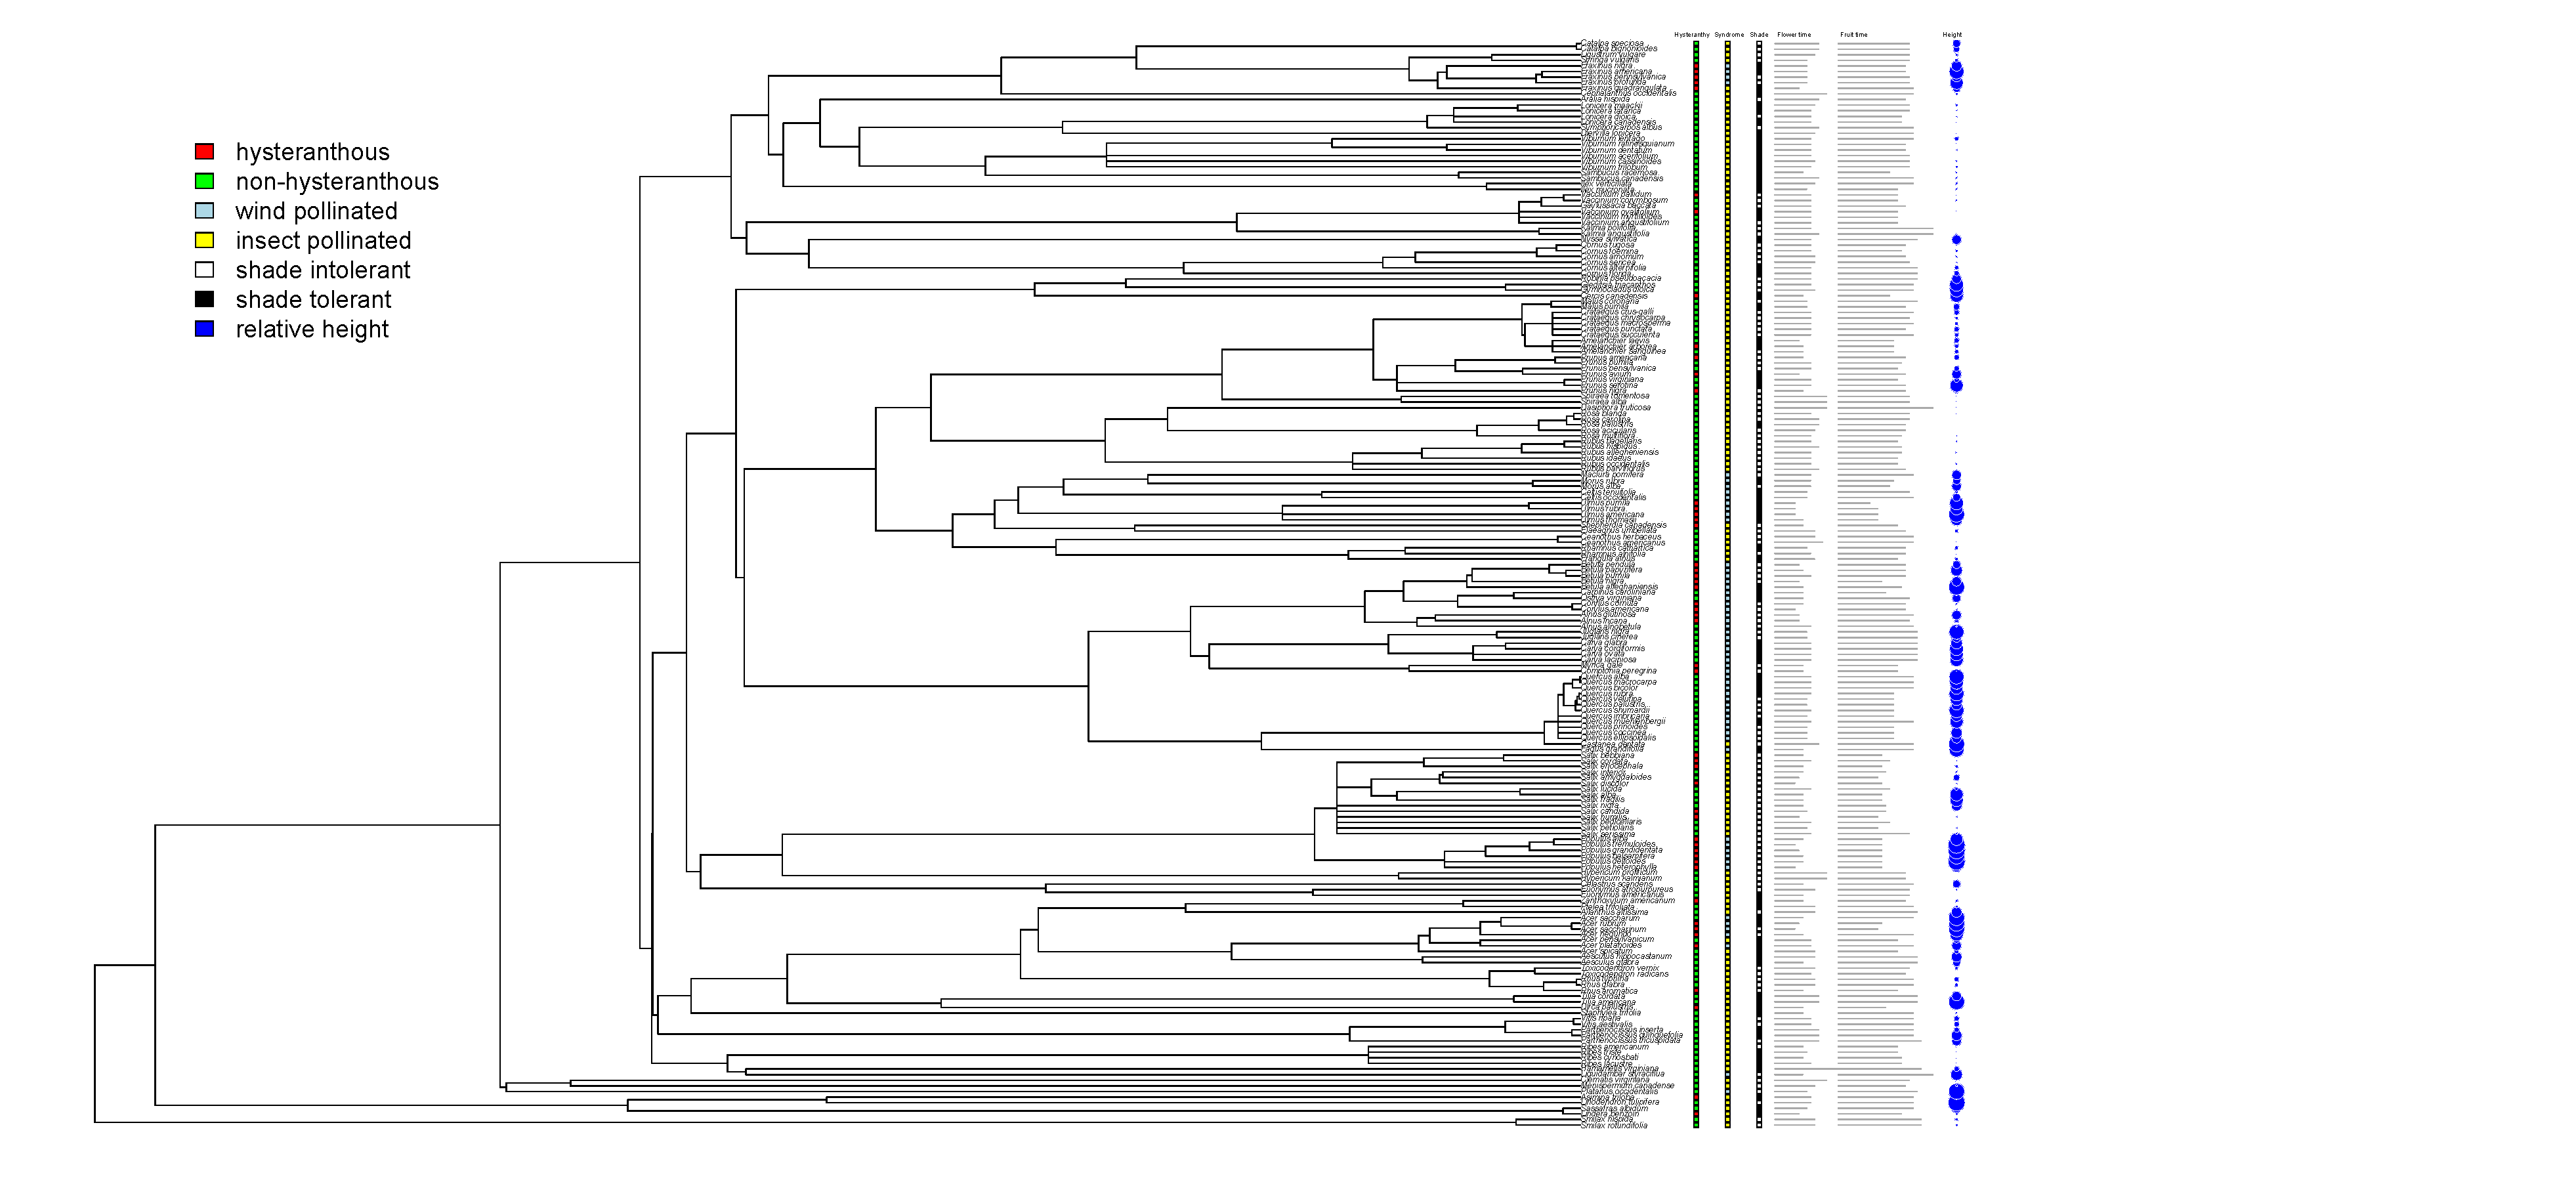
\includegraphics[width=20cm, height=20cm]{../figure/mich_phylo_alltraits.pdf}\\
\caption{I can't figure out how to make this figure more better to look at. Ideas: Just hysteranthy, and/or no tip labels}
\end{figure}
\begin{figure}[h!]
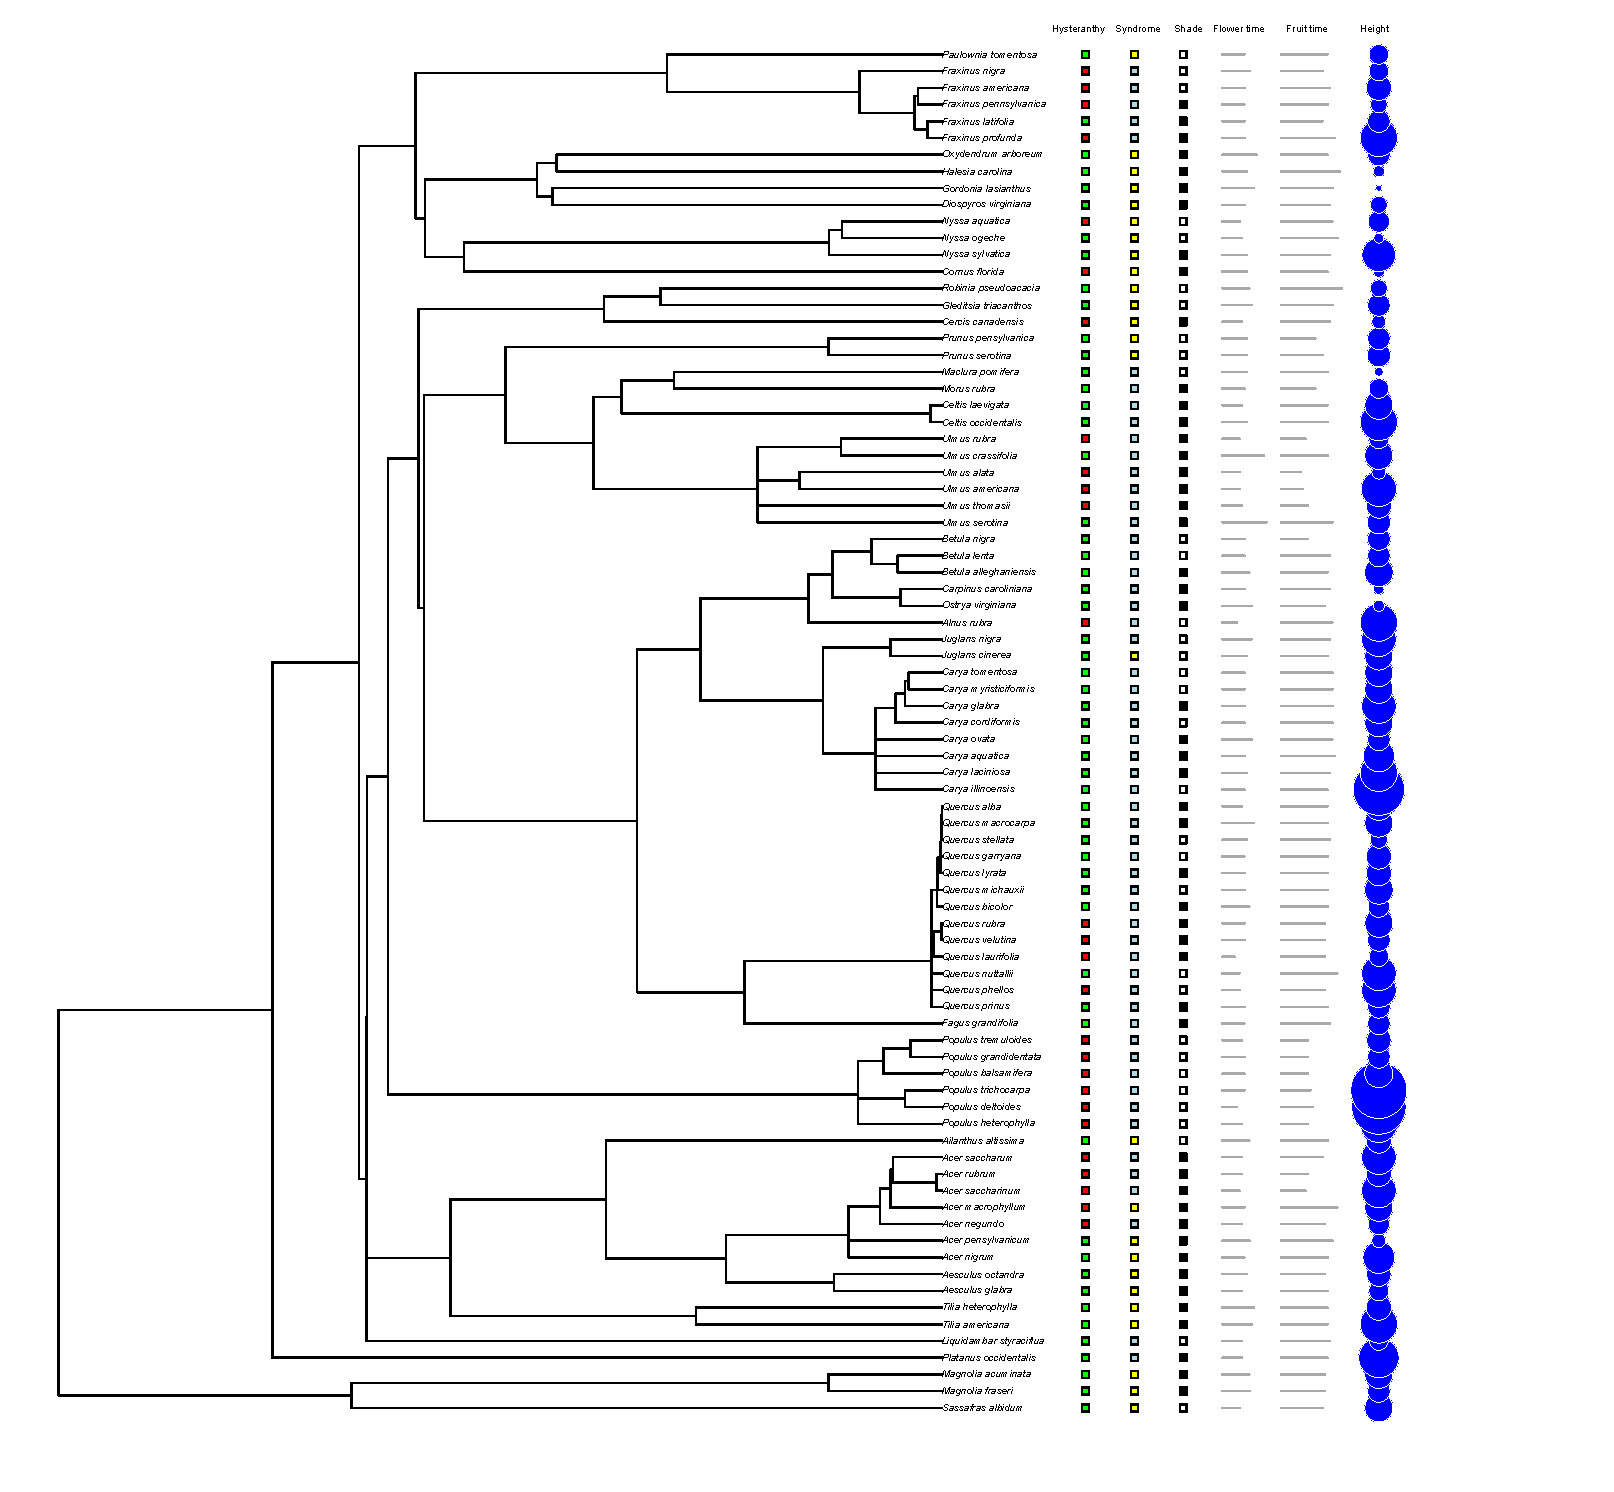
\includegraphics[width=20cm, height=20cm]{../figure/silvics_phylo_alltraits.pdf}\\
\caption{Eventaully these two figures will be side by side}
\end{figure}


\begin{figure}[h!]
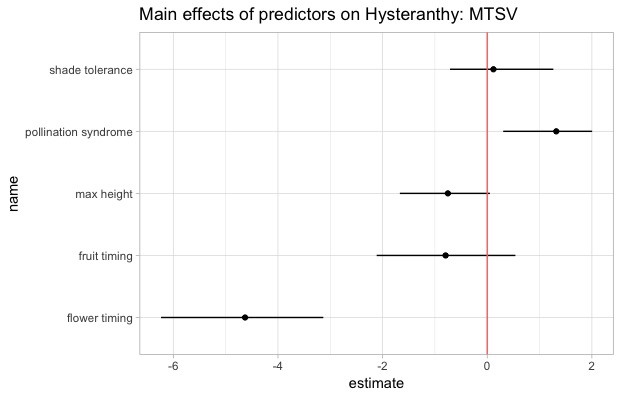
\includegraphics[width=8cm, height=8cm]{../figure/booteffect_MTSV.jpeg}\\
\caption{Eventaully these two figures will be side by side}
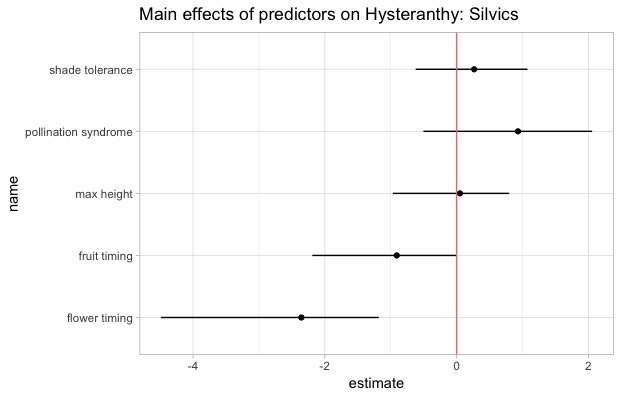
\includegraphics[width=8cm, height=8cm]{../figure/booteffect_sil.jpeg}\\
\caption{Eventaully these two figures will be side by side}
\end{figure}


\end{document}
